%clustering



\begin{frame}
  \frametitle{Clustering - Motivation}
  \begin{itemize}
  	\item Etude des données non étiquetées
  	\item Analyse exploratoire
  	\item Séparation des données en sous-groupes homogènes, appelés \red{clusters}.
  	\item Visualisation
  	\item Première étape pour l'apprentissage supervisé
  \end{itemize}
\end{frame}


\begin{frame}
  \frametitle{Clustering - Exemples}
  \begin{itemize}
  	\item utilisateurs qui ont des comportements similaires 
  	\item communautés sur un réseau social
  	\item motifs récurrents dans des transactions financières
  	\item des pixels d’un même objet dans une image (segmentation d’image)
  	\item des patients dont la maladie s’explique par un même profil génétique
  \end{itemize}
\end{frame}

\begin{frame}
\frametitle{Critère de qualité 1/5}
\begin{itemize}
	\item Définition centroïde du cluster $\cset$: $\muvec_{\cset} = \frac{1}{\cset}\sum_{\xvec \in \cset}\xvec$
	\item Définition médoïde du cluster $\cset$: $\mvec_{\cset} = \argmin_{\xvec \in \cset}d(\xvec, \muvec_{\cset})$
	\item \red{Homogénéité} d'un cluster $k$: 
	\begin{equation*}
	T_k = \frac{1}{|\cset_k|} \sum_{\xvec \in \cset_k} d(\xvec, \muvec_k)
	\end{equation*}
	\item Homogénéité d'un clustering : 
	\begin{equation*}
	T = \frac1K\sum_{k=1}^{K}T_k
	\end{equation*}
\end{itemize}
\end{frame}

\begin{frame}
\frametitle{Critère de qualité 2/5}
\begin{itemize}
	\item Séparabilité des clusters $k$ et $l$ : 
	\begin{equation*}
	s_{kl} = d(\muvec_k, \muvec_l)
	\end{equation*}
	\item Séparabilité globale : 
	\begin{equation*}
	S = \frac{2}{K(K-1)}\sum_{k=1}^{K-1}\sum_{l=k+1}^{K}s_{kl}
	\end{equation*}
\end{itemize}
\end{frame}

\begin{frame}
\frametitle{Critère de qualité 3/5}
\begin{itemize}
	\item Critère de Davis-Bouldin (homogénéité et séparabilité ensemble): 
	\begin{equation*}
	D_k = \max_{l\neq k} \frac{T_k + T_l}{S_{kl}}
	\end{equation*}
	\item Critère de Davis-Bouldin pour un clustering entier : 
	\begin{equation*}
	D = \frac1K \sum_{k=1}^{K}D_k
	\end{equation*}
\end{itemize}
\end{frame}

\begin{frame}
\frametitle{Critère de qualité 4/5}
\begin{itemize}
	\item Coefficient de silhouette. On note d'abord $a(\xvec)$ comme la moyenne des distances de $\xvec$ et des autres points dans le cluster $k(\xvec)$ auquel $\xvec$ est assigné. 	
	\begin{equation*}
	a(\xvec) = \frac{1}{|\cset_{k(\xvec)}| - 1} \sum_{\uvec \in \cset_{k(\xvec)}}d(\xvec, \uvec)
	\end{equation*}
	\item La valeur $b(\xvec)$ correspond à la même expression, mais calculée pour le cluster autre que $k(\xvec)$, pour lequel la valeur est minimale: 	
	\begin{equation*}
	b(\xvec) = \min_{l\neq k(\xvec)}\frac{1}{|\cset_l|} \sum_{u \in \cset_l}d(\uvec, \xvec)
	\end{equation*}
\end{itemize}
\end{frame}

\begin{frame}
\frametitle{Critère de qualité 5/5}
\begin{itemize}
	\item Avec $a$ et $b$ définis ainsi, nous pouvons définir le coefficient de silhouette pour le point $\xvec$ : 
	\begin{equation*}
	s(\xvec) = \frac{b(\xvec)-a(\xvec) }{\max{(b(\xvec), a(\xvec))}  }
	\end{equation*}
	\item Finalement, le \red{coefficient de silhouette} pour le clustering est :
	\begin{equation*}
	s = \frac1n \sum_{i=1}^{n}s(\xvec^i)
	\end{equation*}

\end{itemize}
\end{frame}

%%%%%%%%%%%%%%%% hierarchical clustering
\begin{frame}
\frametitle{Clustering hiérarchique agglomératif}
\begin{itemize}
\item Commencer avec des points de données individuels en tant que clusters distincts.
\item Fusionner les deux clusters les plus proches.
\item Calculer la nouvelle représentation du cluster unique.
\item Répéter cela jusqu'à ce qu'il n'y ait plus rien à fusionner.
\end{itemize}
\end{frame}

\begin{frame}
\frametitle{Clustering hiérarchique divisif}
\begin{itemize}
\item Commencer avec un seul cluster.
\item Diviser le cluster en deux selon une heuristique quelconque.
\item Répéter cela jusqu'à ce qu'on ait des points individuels.
\item Ici, nous traitons uniquement des méthodes de clustering hiérarchique agglomératif (beaucoup plus répondu). 
\end{itemize}
\end{frame}

\begin{frame}
\frametitle{Éléments du clustering hiérarchique}
\begin{itemize}
\item Distance entre points
\item Une règle de fusion de clusters (fonction d'agglomeration)
\end{itemize}
\end{frame}

\begin{frame}
\frametitle{Les distances entre points}
La distance est une fonction 
\begin{equation*}
d: \mathcal{X} \times \mathcal{X} \mapsto \RR^{+} 
\end{equation*}
qui remplit les conditions suivantes : 
\begin{itemize}
\item Symmétrie : $d(a, b) = d(a, b)$
\item Séparation : $d(a, b) \Leftrightarrow a=b$
\item Inégalité triangulaire : $d(a,b) \leq d(a,c) + d(c,b)$
\end{itemize}
\end{frame}

\begin{frame}
\frametitle{Distances entre points}
\begin{itemize}
\item Distance Euclidienne: $d^2(\xvec_i, \xvec_j) = \langle \xvec_i-\xvec_j, \xvec_i-\xvec_j \rangle = \sum_k(x_{i,k}-x_{j,k})^2$
\item Distance Manhattan: $d(\xvec_i, \xvec_j) = \sum_k|x_{i,k}-x_{j,k}|$
\item Distance Euclidienne généralisée : $d^2(\xvec_i, \xvec_j) = (\xvec_i - \xvec_j)^TA(\xvec_i - \xvec_j)$ (exemple: distance Mahalanobis, avec $A=\Sigma^{-1}$)
%\item Distance basée sur la correlation : $d(\xvec_i, \xvec_j) = \frac{1}{2} - \frac{1}{2}\ro(\xvec_i, \xvec_j)$
%\item Distance cosinus : $d(\xvec_i, \xvec_j) = \frac{1}{2} - \frac{1}{2}\frac{\angle \xvec_i, \xvec_j \rangle}{\|\xvec_i\|\|\xvec_j\|} $
\end{itemize}
\end{frame}

% \item Single linkage: $d_{A,B} = \min_{(\xvec_i, x_j) \in A \times B}{d(\xvec_i, \xvec_j)}$
% \item Complete linkage: $d_{A,B} = \max_{(\xvec_i, \xvec_j) \in A \times B}{d(\xvec_i, \xvec_j)}$
% \item Average linkage: $d_{A,B} = \frac{1}{N_AN_B} \sum_{(\xvec_i, \xvec_j) \in A \times B} d(\xvec_i, \xvec_j)$
% \item Centroid: $d_{A,B} = d(\mu_A, \mu_B)$ with $\mu_A$, $\mu_B$ the average of $\xvec$ in $A$ and $B$ respectively.  
% \item Ward: $d_{A,B} = \frac{N_AN_B}{N_A+N_B}\|\mu_A - \mu_B\|^2$ with $\mu_A$, $\mu_B$ the average of $\xvec$ in $A$ and $B$ respectively. The ward method chooses the cluster fusion producing the smallest increase in variance. 



\begin{frame}
\frametitle{Fonctions d'agglomération}
\begin{figure}[htb]
  \centering
  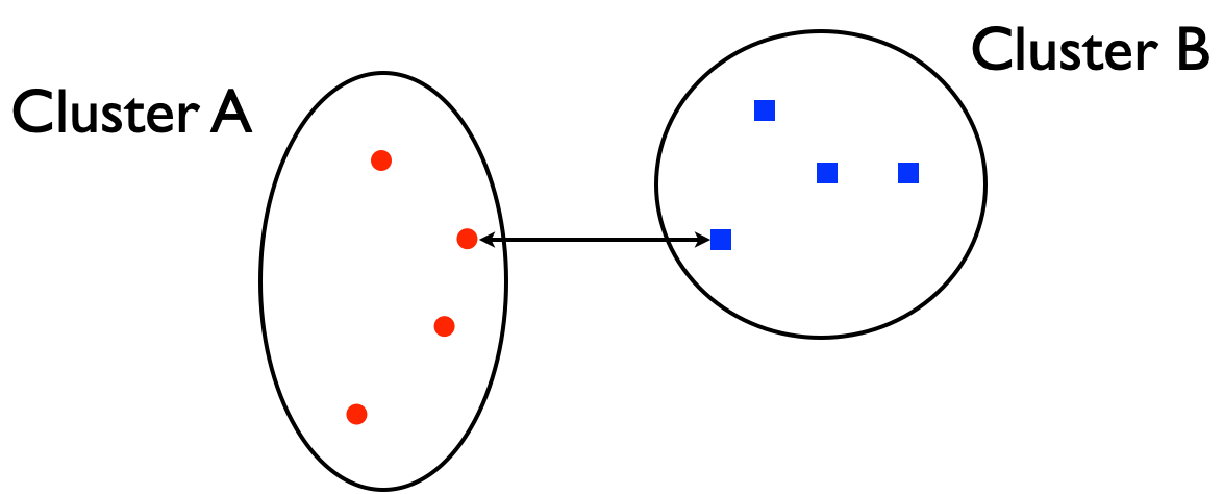
\includegraphics[width=.8\textwidth]{SingleLinkage}
  \caption{Single Linkage}
\end{figure}
Single Linkage: 
\begin{equation*}
d_{A,B} = \min_{(\xvec_i,\xvec_j) \in A \times B}{d(\xvec_i, \xvec_j)}
\end{equation*}

\end{frame}


\begin{frame}
\frametitle{Fonctions d'agglomération}
\begin{figure}[htb]
  \centering
  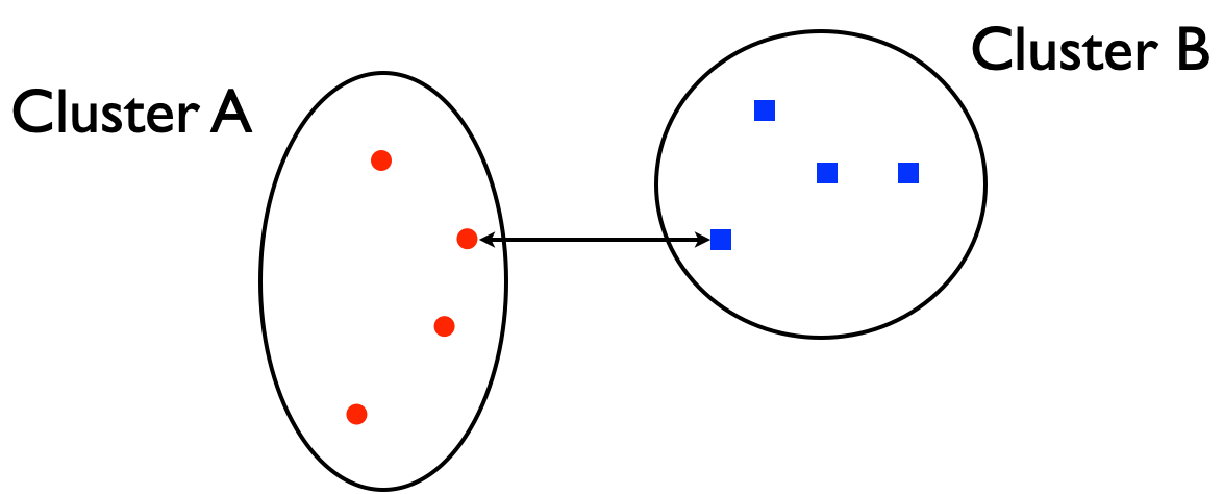
\includegraphics[width=.8\textwidth]{CompleteLinkage}
  \caption{Complete Linkage}
\end{figure}
Complete linkage: $d_{A,B} = \max_{(\xvec_i, \xvec_j) \in A \times B}{d(\xvec_i, \xvec_j)}$
\end{frame}


\begin{frame}
\frametitle{Fonctions d'agglomération}

\begin{figure}[htb]
  \centering
  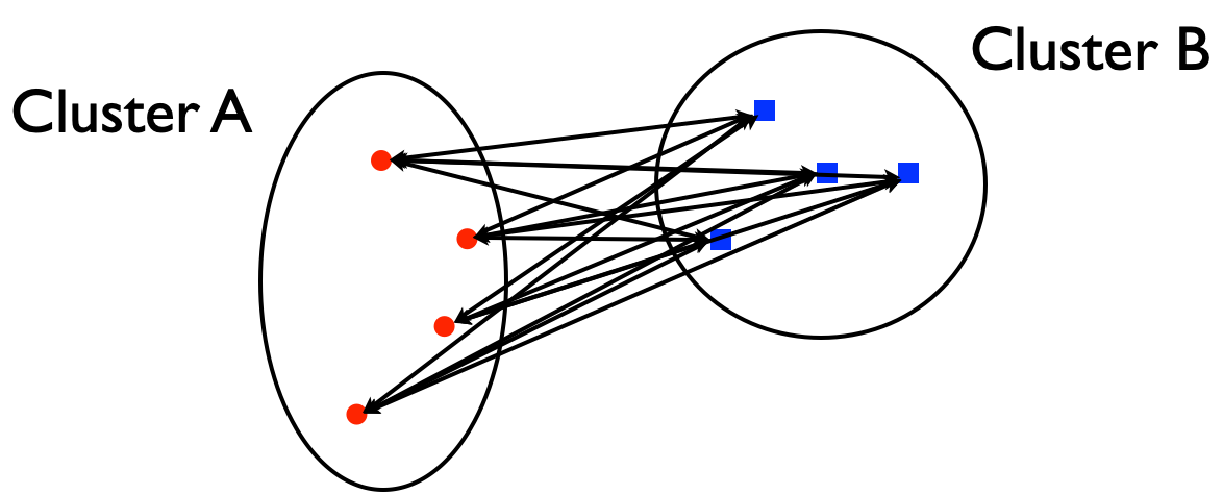
\includegraphics[width=.8\textwidth]{AverageLinkage2}
  \caption{Average Linkage}
\end{figure}
Average linkage: $d_{A,B} = \frac{1}{N_AN_B} \sum_{(\xvec_i, \xvec_j) \in A \times B} d(\xvec_i, \xvec_j)$
\end{frame}



\begin{frame}
\frametitle{Fonctions d'agglomération}

\begin{figure}[htb]
  \centering
  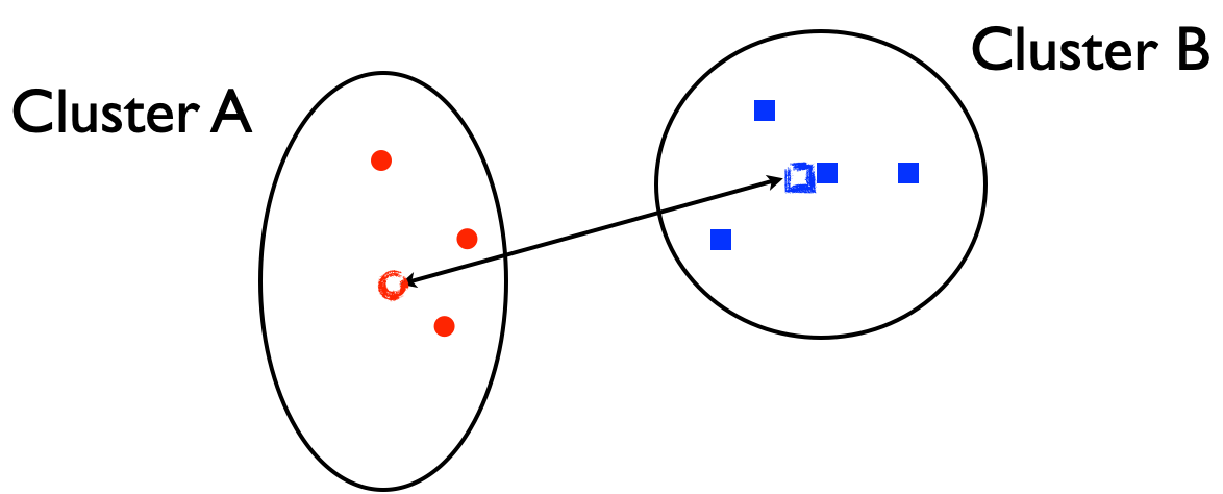
\includegraphics[width=.8\textwidth]{CentroidLinkage}
  \caption{Centroid Linkage}
\end{figure}
Centroid: $d_{A,B} = d(\mu_A, \mu_B)$ with $\mu_A$, $\mu_B$ the average of $\xvec$ in $A$ and $B$ respectively.  
\end{frame}


\begin{frame}
\frametitle{Fonctions d'agglomération}
\begin{figure}[htb]
  \centering
  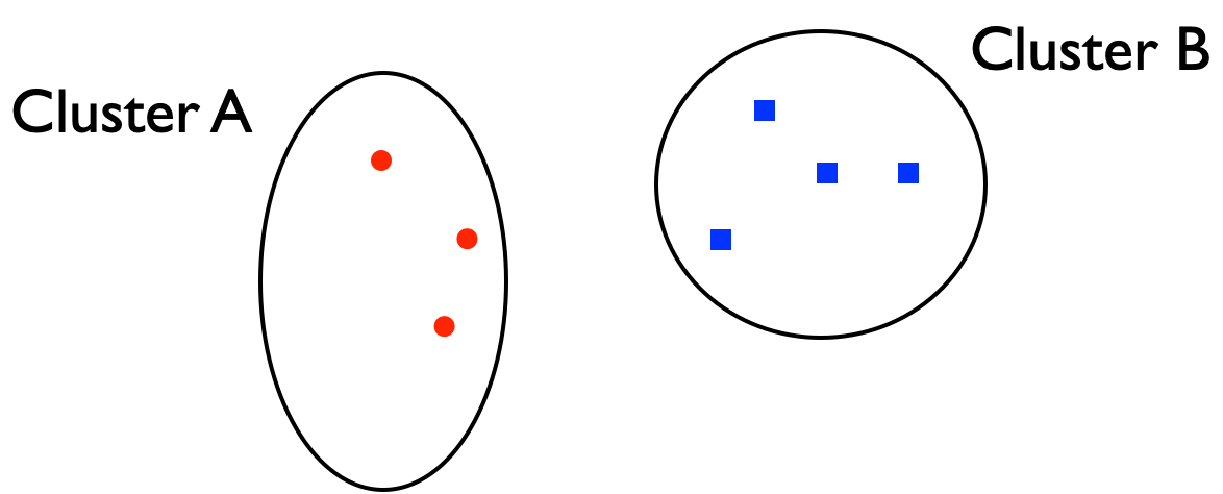
\includegraphics[width=.8\textwidth]{WardLinkage}
  \caption{Ward Linkage}
\end{figure}
Ward: $d_{A,B} = \frac{N_AN_B}{N_A+N_B}\|\overrightarrow{\mu}_A - \overrightarrow{\mu}_B\|^2$
$\overrightarrow{\mu}_A$, $\overrightarrow{\mu}_B$ sont les moyennes de $\xvec$ dans $A$, $B$. La méthode de Ward choisit la fusion qui produit la plus petite augmentation de la variance intra-cluster. 
\end{frame}

\begin{frame}
\frametitle{Clustering hiérarchique : exemple}
\begin{figure}[htb]
  \centering
  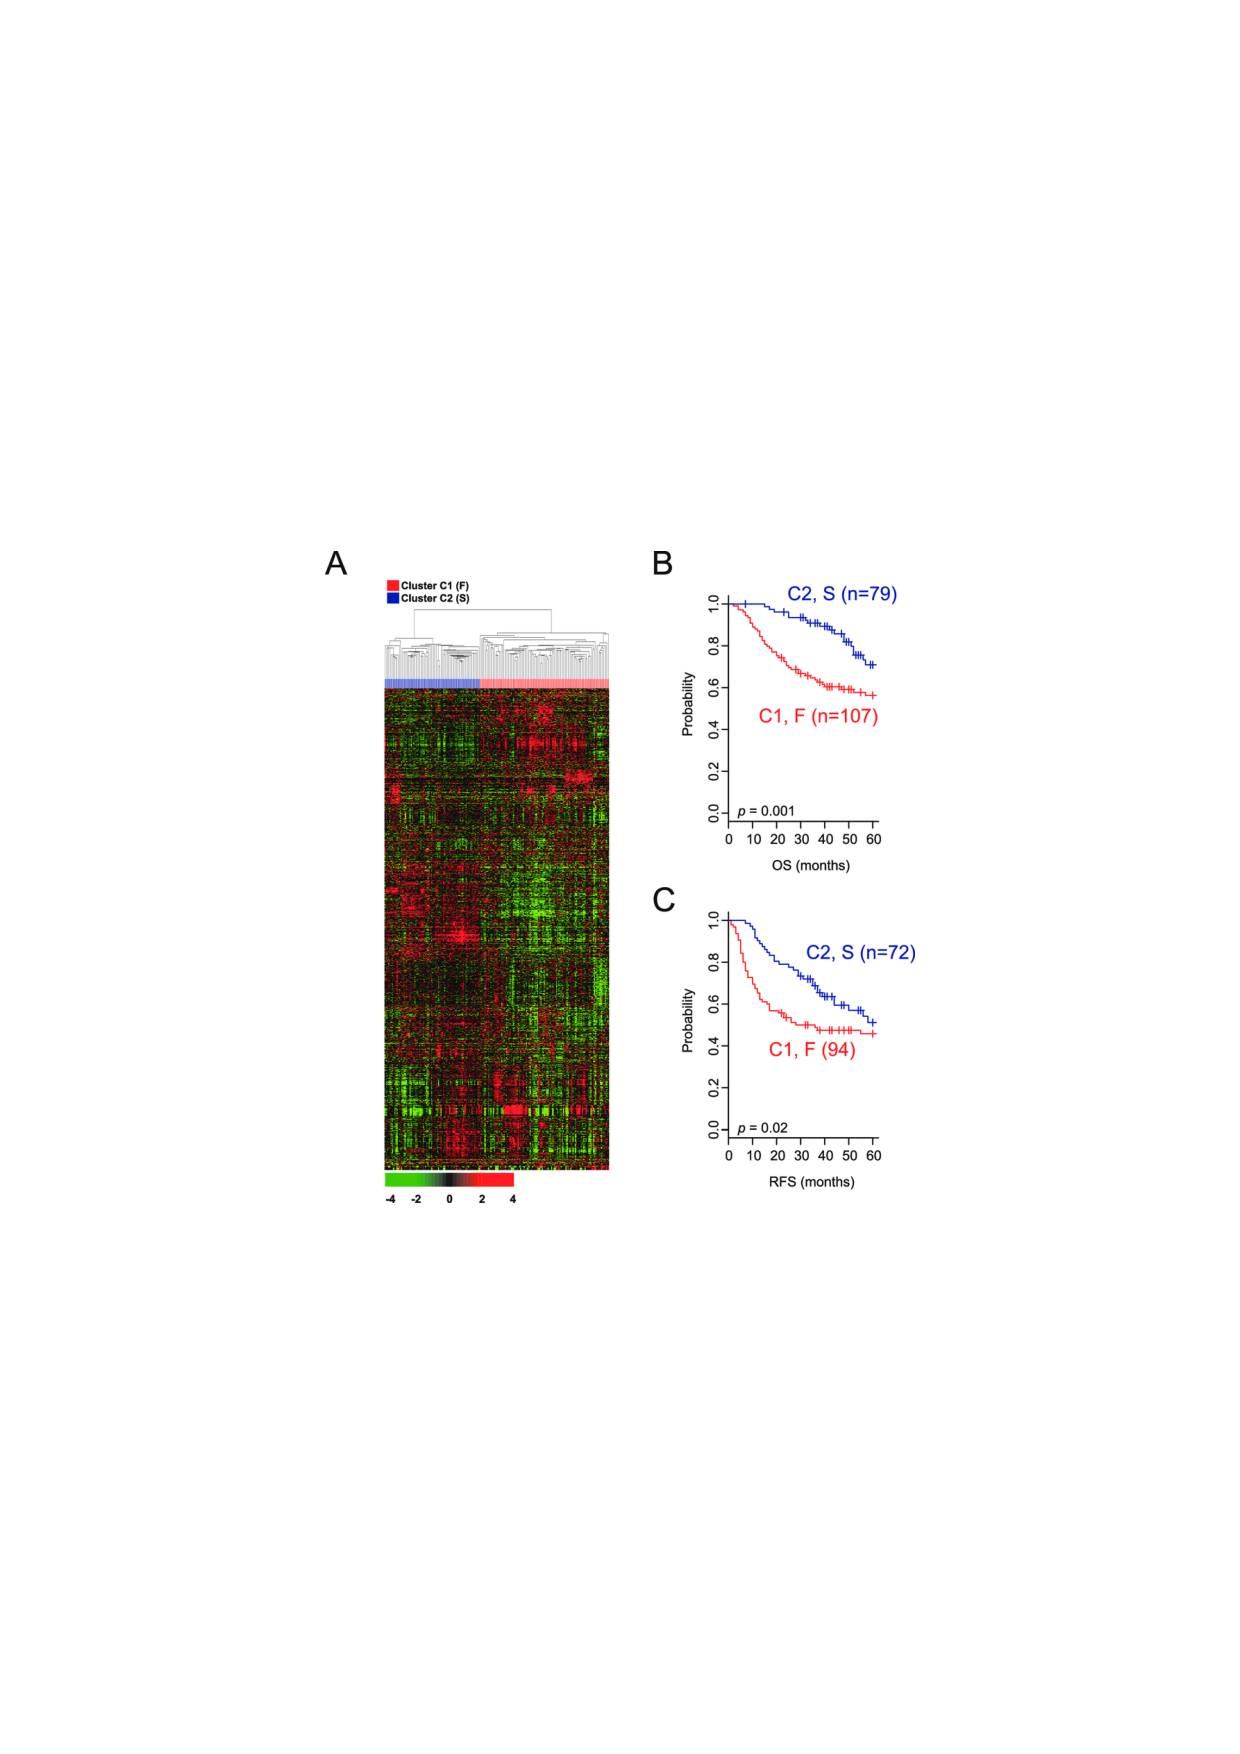
\includegraphics[height=0.7\textheight]{HierarchicalClustering_Example}
  \caption{Exemple: clustering hiérarchique sur des données d'expression génétique dans le cancer du poumon (colonnes : tissue, lignes : gènes)}
\end{figure}
\end{frame}



%%%%%%%%%%%%%%%% k-means
\begin{frame}
\frametitle{Méthode des k-moyennes}
\begin{itemize}
	\item On fixe un nombre $K$ de clusters. 
	\item On essaie de trouver une affectation des points $\xvec_i$ aux clusters afin de minimiser l'intra-cluster variance : 
	\begin{equation*}
	\argmin_{\cset_1, \cset_2, \ldots, \cset_K} \sum_{k=1}^K \sum_{\xvec \in \cset_k} \ltwonorm{\xvec - \muvec}^2
	\end{equation*}
\end{itemize}
\end{frame}

\begin{frame}
\frametitle{Méthode des k-moyennes : algorithme de Lloyd}
\begin{enumerate}
	\item Initialisation : choisir les $\muvec_1, \muvec_2, \ldots, \muvec_K$ parmi les points $\xvec$. 
	\item Affecter chaque observation $\xvec \in \dset$ au centroïde dont elle est le plus proche :
	\begin{equation*}
		k(\xvec^i) = \argmin_{k=1, \ldots, K}\ltwonorm{\xvec^i - \muvec_k}^2
	\end{equation*}
	\item Recalculer les centroïdes $\muvec_k$. 
	\item Répéter jusqu'à ce que les affectations ne changent plus. 
\end{enumerate}
\end{frame}

\begin{frame}
\frametitle{Algorithme de Lloyd - limitations}
\begin{itemize}
\item L'algorithme de Lloyd converge très rapidement. 
\item \blue{Problème} : l'algorithme est glouton (greedy) et peut rester dans un minimum local. \blue{Solution} : répéter l'algorithme $t$ fois et prendre la solution avec la meilleure intra-cluster variance. 
\item \blue{Problème} : dépendance de l'initialisation. \blue{Solution} : placer les centres avec dispersion maximale.
\item \blue{Problème} : les clusters sont nécessairement convexes. \blue{Solution} : l'astuce de noyau peut s'appliquer ici aussi. 
\end{itemize}
\end{frame}

\begin{frame}
\frametitle{k-moyennes: avantages et inconvénients}
  \begin{itemize}
  	\item Avantages : 
  	\begin{itemize}
  		\item rapide
  		\item optimisation globale
  	\end{itemize}
  	\item Inconvénients : 
  	\begin{itemize}
  		\item il faut déterminer $K$
  		\item Problème non-convexe
  		\item Forme convexe des clusters
  	\end{itemize}
  	\item L'algorithme des k-moyennes est l'un des plus répandus en apprentissage non-supervisé. 
  \end{itemize}
\end{frame}

\begin{frame}
\frametitle{DBSCAN - Motivation}
\begin{figure}[htb]
  \centering
  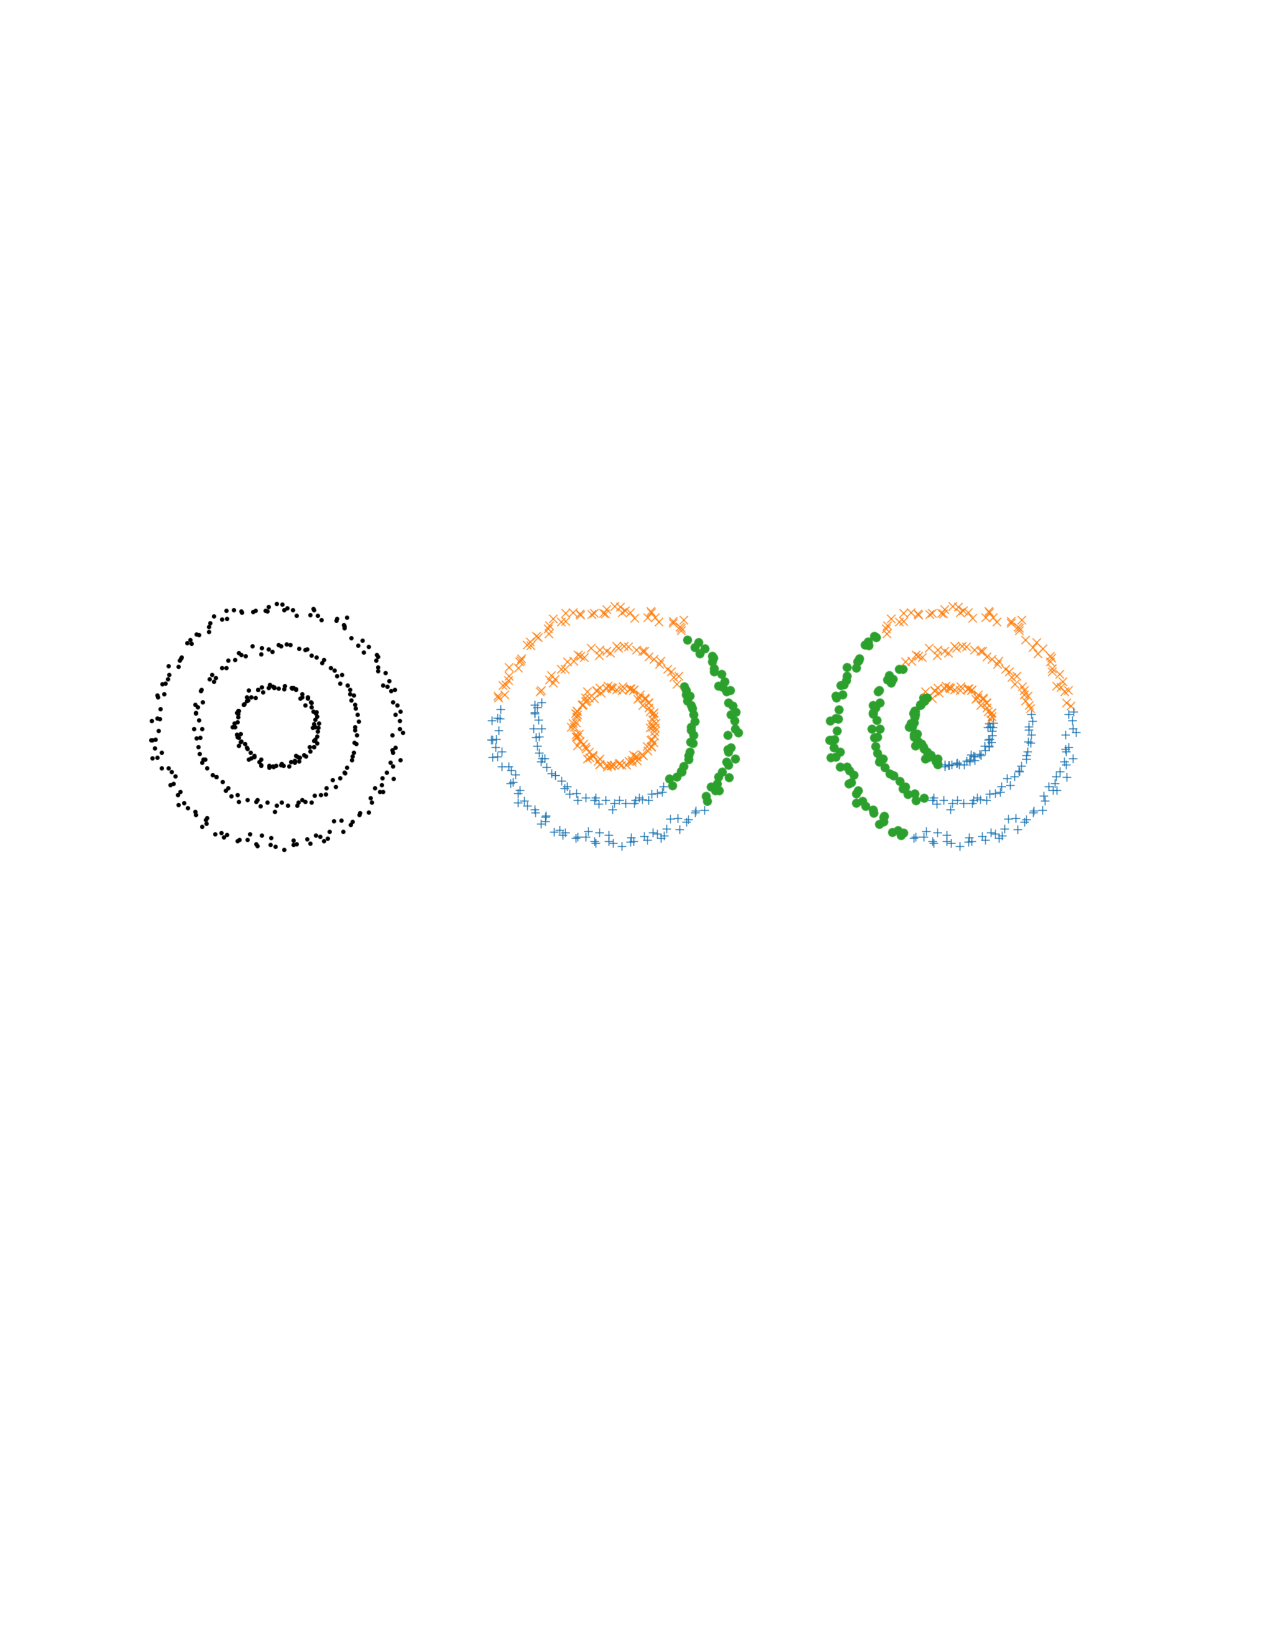
\includegraphics[width=.8\textwidth]{dbscan_motivation}
  \caption{Échec d'algorithmes sur le problème de cercles concentriques}
\end{figure}
\red{Idée : utiliser les densités locales}
\end{frame}



\begin{frame}
\frametitle{DBSCAN - Algorithme}
\begin{itemize}
	\item On définit : 
	\begin{itemize}
		\item Un voisinage $\nset_{\epsilon}$ (boule autour de chaque point, avec rayon $\epsilon$)
		\item Un nombre minimal de voisins $n_{min}$ dans le voisinage. 
	\end{itemize}
	\item On considère chaque point comme aberrant (outlier), s'il ne remplit pas le critère du nombre minimal. 
	\item On itère sur les points $\xvec \in \dset$, et on ajoute tous les points qui sont atteignables de $\xvec$ avec un chemin qui ne requiert pas de distance entre points plus grande que $\epsilon$. 
\end{itemize}
\end{frame}

\begin{frame}
\frametitle{DBSCAN - chemin / résultats}
\begin{figure}[htb]
  \centering
  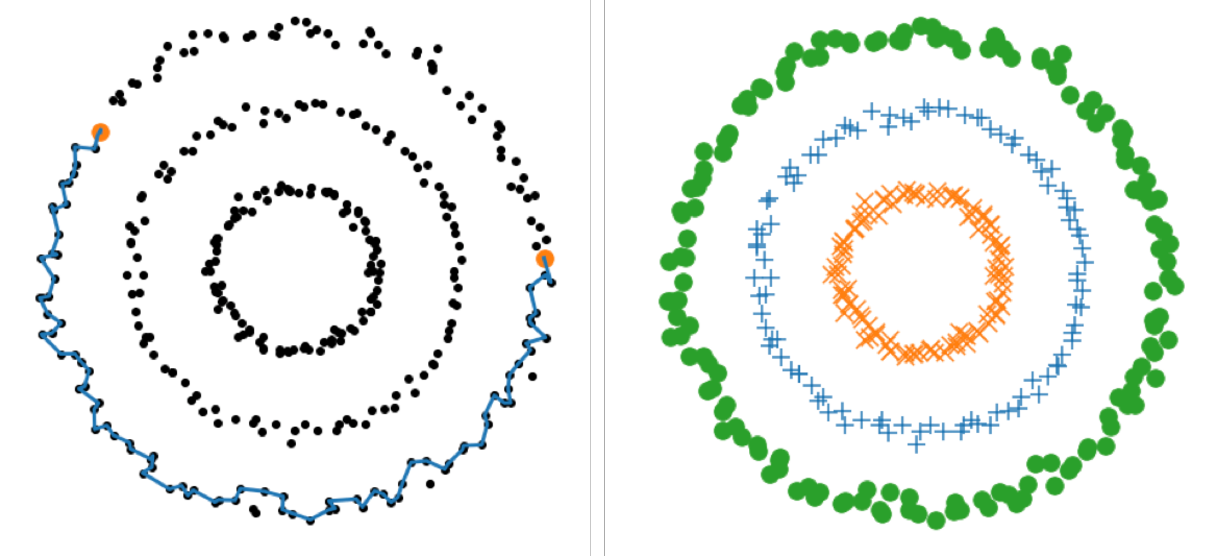
\includegraphics[width=.8\textwidth]{dbscan}
\end{figure}
\begin{itemize}
	\item À gauche, on voit le chemin qui est utilisé dans l'algorithme. 
\end{itemize}
\end{frame}

\begin{frame}
\frametitle{DBSCAN : avantages et inconvénients}
  \begin{itemize}
  	\item Avantages : 
  	\begin{itemize}
  		\item n'impose pas de forme particulière
  		\item simple, pas de définition du nombre de clusters
  		\item robustesse aux données aberrantes
  	\end{itemize}
  	\item Inconvénients : 
  	\begin{itemize}
  		\item ne sait pas gérer des écarts
  		\item peu de résultats théoriques
  		\item pas applicable en très haute dimension (à cause de la définition de $\nset_{\epsilon}$)
  	\end{itemize}
  \end{itemize}
\end{frame}


\begin{frame}
\frametitle{Conclusion (clustering)}
\begin{itemize}
	\item Le clustering, ou partitionnement de données, cherche à identifier des classes sans utiliser d’étiquettes
	\item La qualité d’une partition peut s’évaluer sur des critères de séparabilité et d’homogénéité
	\item k-moyennes: Il permet de trouver efficacement K clusters convexes.
	\item DBSCAN : détection des formes non-convexes (en basse dimension). 
\end{itemize}
\end{frame}

\begin{frame}
\frametitle{Conclusion générale - avant de commencer}
\begin{itemize}
\item Spécification du problème : 
\begin{itemize}
	\item supervisé ou non-supervisé ? 
	\item régression ou classification ? 
\end{itemize}
\item Quantification pour la mise en place:
\begin{itemize}
	\item combien de descripteurs ($p$) ? 
	\item combien d'échantillons annotés ($n$) ? 
	\item combien d'échantillons non-annotés ?
\end{itemize}
\end{itemize}
\end{frame}

\begin{frame}
\frametitle{Conclusion générale - avant de commencer}
\begin{itemize}
	\item Exigences supplémentaires : 
	\begin{itemize}
		\item interprétabilité des modèles
		\item robustesse 
		\item compromis sensibilité / précision
		\item biais et perturbations potentiels
	\end{itemize}
\end{itemize}
\end{frame}

\begin{frame}
\frametitle{Conclusion générale - méthodes non-supervisées}
\begin{itemize}
	\item Exploration graphique des données : 
	\begin{itemize}
		\item Réduction de dimensions (ACP, t-SNE)
		\item Clustering pour trouver des groupes
	\end{itemize}
	\item Le but est comprendre les distributions des données et éventuellement d'identifier des groupes. 
	\item Visualisation joue souvent un rôle clé pendant cette phase exploratoire.
\end{itemize}
\end{frame}

\begin{frame}
\frametitle{Conclusion générale - problèmes supervisés}
\begin{itemize}
	\item Si $n \gg p$ : 
	\begin{itemize}
		\item des méthodes classiques comme la $LDA$ ou la régression logistique peuvent s'appliquer. 
		\item Problème potentiel : corrélation des descripteurs. Solution possible : sélectionner les descripteurs, ou bien appliquer une $ACP$. 
		\item Tester l'effet d'une régularisation. 
	\end{itemize}
	\item Si $p > n$ (et même si $p \gg n$): 
	\begin{itemize}
		\item les $SVM$ ou les $RF$ sont préférables. 
		\item la régularisation se fait avec la norme $L_2$ des paramètres pour les $SVM$ et par ensembling pour les $RF$. 
	\end{itemize}
\end{itemize}
\end{frame}

% \begin{frame}
% \frametitle{Conclusion générale - problèmes supervisés}
% \begin{itemize}
% 	\item Fixer les hyper-paramètres par validation croisée. 
% 	\item Évaluation de performance sur un jeu de données pas utilisé pour l’entraînement ou la sélection de modèles.
% 	\item Tests supplémentaires concernant la robustesse, le temps de calcul, etc. 
% \end{itemize}
% \end{frame}



% \begin{frame}
% \frametitle{Conclusion générale}
% \begin{itemize}
% 	\item 
% 	\item La qualité d’une partition peut s’évaluer sur des critères de séparabilité et d’homogénéité
% %— Le clustering hiérarchique partitionne les données de manière itérative. Son résultat peut être vi- sualisé sur un dendrogramme.
% 	\item k-moyennes: Il permet de trouver efficacement K clusters convexes.
% %— Laversionànoyaudelaméthodedesk-moyennespermetdel’appliquerpourdécouvrirdesclusters non convexes.
% 	\item DBSCAN : détection des formes non-convexes (en basse dimension). 
% %— Le clustering par densité permet d’identifier des régions denses du jeu de données, c’est-à-dire des observations qui peuvent former un ensemble non convexe mais qui sont proches les unes des autres.
% \end{itemize}
% \end{frame}


